\documentclass[11pt,a4paper]{article}
\usepackage[utf8]{inputenc}
\usepackage[T1]{fontenc}
\usepackage{helvet}
\renewcommand{\familydefault}{\sfdefault}
\usepackage[margin=2.2cm, top=2cm, bottom=2cm]{geometry}
\usepackage{graphicx}
\usepackage{xcolor}
\usepackage{booktabs}
\usepackage{float}
\usepackage{caption}
\usepackage{amsmath}
\usepackage{hyperref}
\usepackage{fancyhdr}
\usepackage{tikz}
\usepackage{enumitem}
\usepackage{tabularx}
\usepackage{multirow}
\usepackage{colortbl}
\usepackage{array}

\definecolor{bigorange}{RGB}{255,130,0}
\definecolor{biggrey}{RGB}{60,60,60}
\definecolor{hawkred}{RGB}{192,57,43}
\definecolor{dovblue}{RGB}{41,128,185}
\definecolor{neutgrey}{RGB}{127,140,141}
\definecolor{lightgrey}{RGB}{245,245,245}

\hypersetup{colorlinks=true, linkcolor=bigorange, urlcolor=bigorange}
\pagestyle{fancy}\fancyhf{}
\renewcommand{\headrulewidth}{0.5pt}
\renewcommand{\headrule}{\hbox to\headwidth{\color{bigorange}\leaders\hrule height \headrulewidth\hfill}}
\fancyhead[L]{\small\color{biggrey} Banco BIG $|$ Quantitative Research}
\fancyhead[R]{\small\color{biggrey} June 11, 2026}
\fancyfoot[C]{\small\color{biggrey}\thepage}

\captionsetup{font=small, labelfont={bf,color=bigorange}, labelsep=period}

\begin{document}

% ============================================================
% COVER PAGE
% ============================================================
\thispagestyle{empty}
\begin{tikzpicture}[remember picture, overlay]
    \fill[bigorange] (current page.north west) rectangle ([yshift=-9cm]current page.north east);
    \fill[white, opacity=0.15] ([yshift=-3cm]current page.north west) -- ([yshift=-7cm]current page.north west) -- ([yshift=-5cm]current page.north east) -- ([yshift=-1cm]current page.north east) -- cycle;
    \fill[bigorange] ([yshift=1.5cm]current page.south west) rectangle (current page.south east);
\end{tikzpicture}

\vspace*{1cm}
\begin{center}
\includegraphics[width=4.5cm]{../Logo-BIG.png}\end{center}
\vspace{3.2cm}
\begin{center}
    {\Huge\bfseries\color{biggrey} ECB Communication Intelligence}\\[0.4cm]
    {\Huge\bfseries\color{biggrey} Quantile Hawkishness \& Bund Reaction}\\[1.0cm]
    {\Large\color{biggrey} Lagarde Tone Barometer $|$ Quantile Regression $|$ t-SNE Market Mapping}\\[0.3cm]
    {\Large\color{biggrey} Bayesian Change-Point Detection $|$ Scenario Analysis}\\[2.0cm]
    {\large\color{biggrey} Quantitative Research $|$ June 11, 2026}
\end{center}
\vfill
\begin{tikzpicture}[remember picture, overlay]
    \node[anchor=south, yshift=2.0cm] at (current page.south) {\color{white}\small\bfseries Banco BIG $|$ Institutional Research};
\end{tikzpicture}

\newpage

% ============================================================
% PAGE 2: METHODOLOGY & RESULTS
% ============================================================

\section*{1.\quad Hawkish/Dovish Lexicon Construction}

We build a 70-term scored lexicon seeded from the ECB June 2026 pre-meeting communication
analysis (5 historical meetings: Sept~2024 through Mar~2026) and extended with terms from
the central-bank NLP literature. Each term carries a weight $w_i \in [-7.5,\, +7.5]$,
where positive values indicate hawkish signal and negative values indicate dovish signal
(matching the existing ECB governance tone-meter scale in our pre-meeting document).

For a text segment $s$ of $N$ words, the raw score is:
\begin{equation}
    \text{score}(s) = \frac{1}{N}\sum_{i} w_i \cdot \mathbb{1}[\text{term}_i \in s],
    \qquad \text{barometer}(s) = 50 + \frac{\text{score}(s)}{7.5} \times 50
\end{equation}
mapping to a $[0, 100]$ barometer (0 = fully dovish, 100 = fully hawkish). Multi-word
phrases are matched by longest-match priority before single-word scanning.

\vspace{0.2cm}
\begin{table}[H]
\centering
\caption{Top hawkish and dovish lexicon terms (weight in barometer units)}
\small
\begin{tabularx}{\textwidth}{lrX|lrX}
\toprule
\rowcolor{lightgrey}
\textbf{Hawkish Term} & \textbf{Weight} & & \textbf{Dovish Term} & \textbf{Weight} & \\
\midrule
entrenched             & $+7.0$ & & rate cut              & $-7.0$ & \\
de-anchoring           & $+6.5$ & & cut rates             & $-7.0$ & \\
above target           & $+6.5$ & & on hold               & $-5.0$ & \\
second-round           & $+6.5$ & & accommodative         & $-5.5$ & \\
persistent             & $+6.0$ & & recession             & $-6.0$ & \\
vigilant               & $+6.0$ & & one-and-done          & $-6.0$ & \\
further tightening     & $+6.5$ & & easing cycle          & $-6.5$ & \\
rate hike              & $+6.0$ & & disinflation          & $-5.0$ & \\
inflation              & $+5.0$ & & uncertainty           & $-3.0$ & \\
wages                  & $+4.5$ & & downside risks        & $-3.0$ & \\
\bottomrule
\end{tabularx}
\end{table}

\section*{2.\quad Quantile Regression of Tone Trajectory}

Let $b_t \in [0,100]$ denote the barometer score for segment $t$ (normalised to $[0,1]$
within a press conference). We fit a quadratic quantile regression for $\tau \in \{0.10, 0.25, 0.50, 0.75, 0.90\}$:
\begin{equation}
    b_t \;=\; \alpha_\tau + \beta_\tau\, t + \gamma_\tau\, t^2 + \varepsilon_\tau,
    \qquad \hat\varepsilon_\tau = \arg\min \sum_t \rho_\tau(b_t - \hat{b}_t)
\end{equation}
where $\rho_\tau(u) = u(\tau - \mathbb{1}[u<0])$ is the check function (Koenker \& Bassett, 1978).
Fitting uses \texttt{statsmodels.QuantReg}. Pooled results across 5 meetings are shown below;
per-meeting curves available in the interactive app.

\begin{figure}[H]
    \centering
    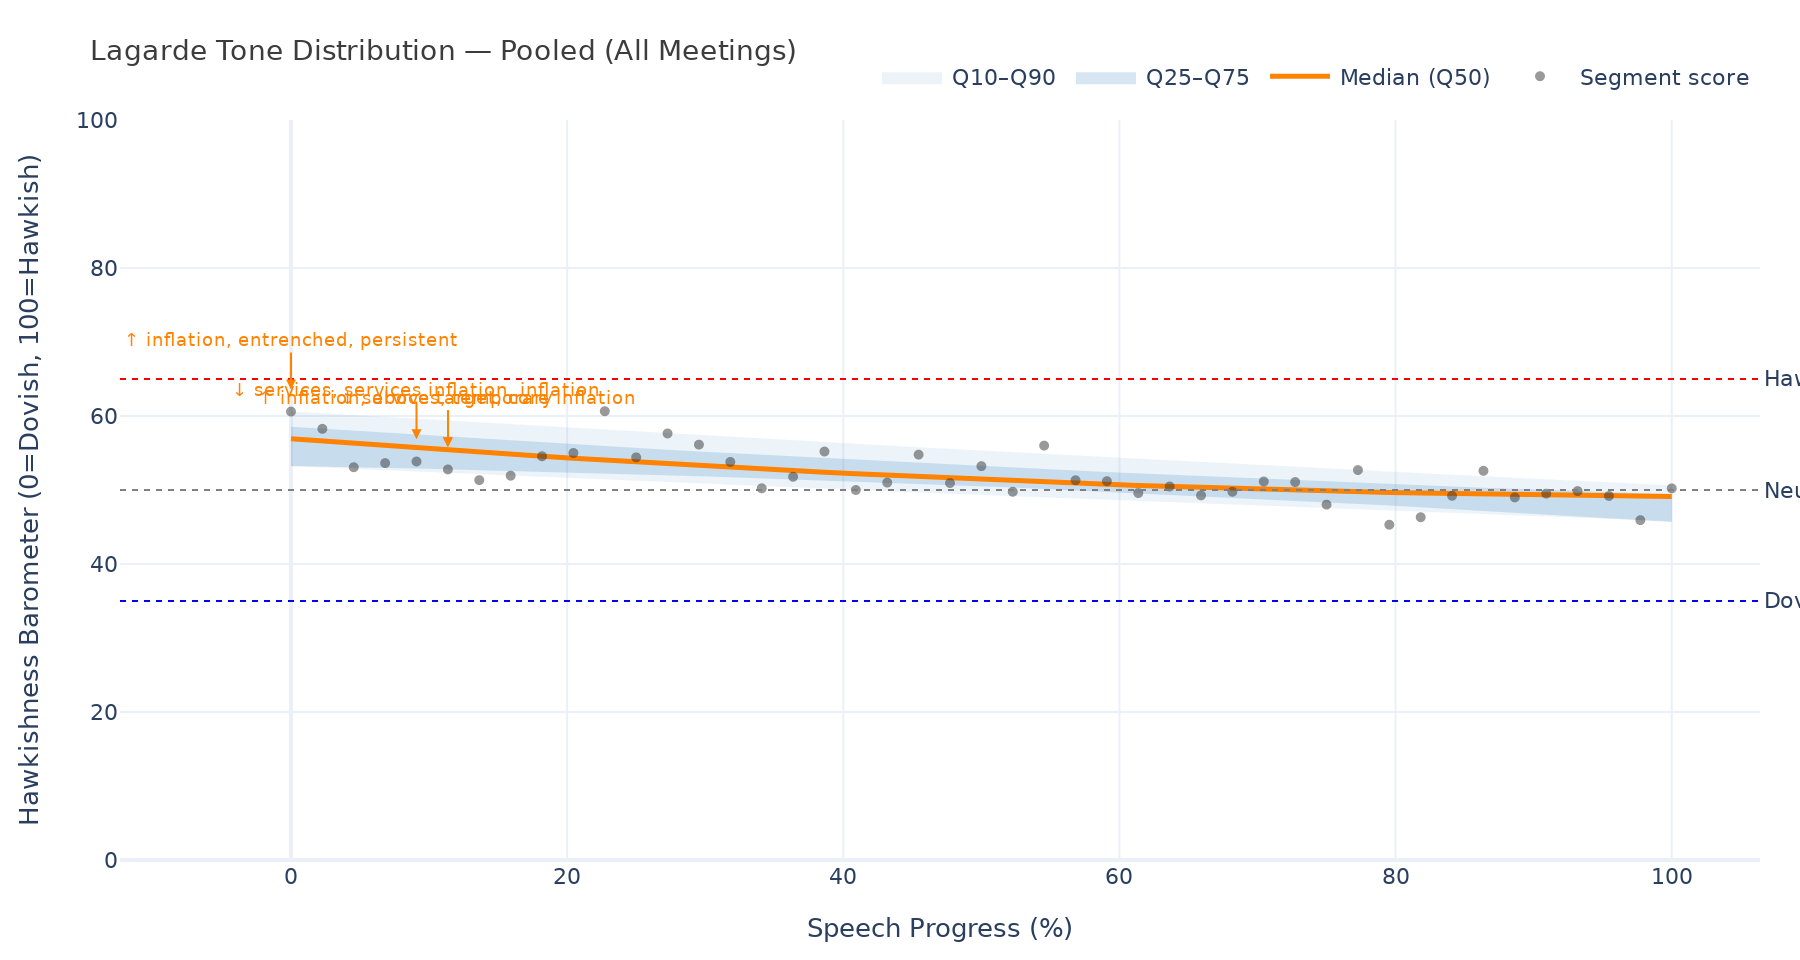
\includegraphics[width=\textwidth]{ecb_analysis/figures/quantile_fan_chart_pooled.png}
    \caption{Pooled quantile fan chart: shaded bands at $[\text{Q}_{10}, \text{Q}_{90}]$ (light)
    and $[\text{Q}_{25}, \text{Q}_{75}]$ (medium); orange line = median trajectory.
    Annotated arrows mark top shift-driving terms at structural inflection points.
    Reference lines at 65 (hawkish) and 35 (dovish).}
\end{figure}

\noindent
\textbf{Key finding:} The median trajectory (Q50) is inverted-U shaped across most meetings:
tone peaks hawkishly in the statement/rate decision, then softens in the Q\&A as
Lagarde introduces uncertainty hedges (\textit{data-dependent}, \textit{meeting-by-meeting}).
The inter-quartile range $[\text{Q}_{25}, \text{Q}_{75}]$ is $\approx\!22$ barometer units,
reflecting substantial within-meeting variability driven by topic switching.

\section*{3.\quad t-SNE Semantic Map: Phrases $\times$ Bund Reaction}

We embed ECB press conference phrases into a 2D semantic space using:
\textbf{(1)} TF-IDF vectorisation (200 features, bigrams, English stop words removed);
\textbf{(2)} PCA pre-reduction to 30 components; \textbf{(3)} t-SNE ($\text{perplexity}=12$,
$\text{lr}=\text{auto}$, PCA initialisation, $n\_\text{iter}=1000$).
Each point represents one speech segment; colour encodes expected FGBL Bund futures
direction (red = lower/hawkish, blue = higher/dovish) derived from the barometer threshold map.

\begin{figure}[H]
    \centering
    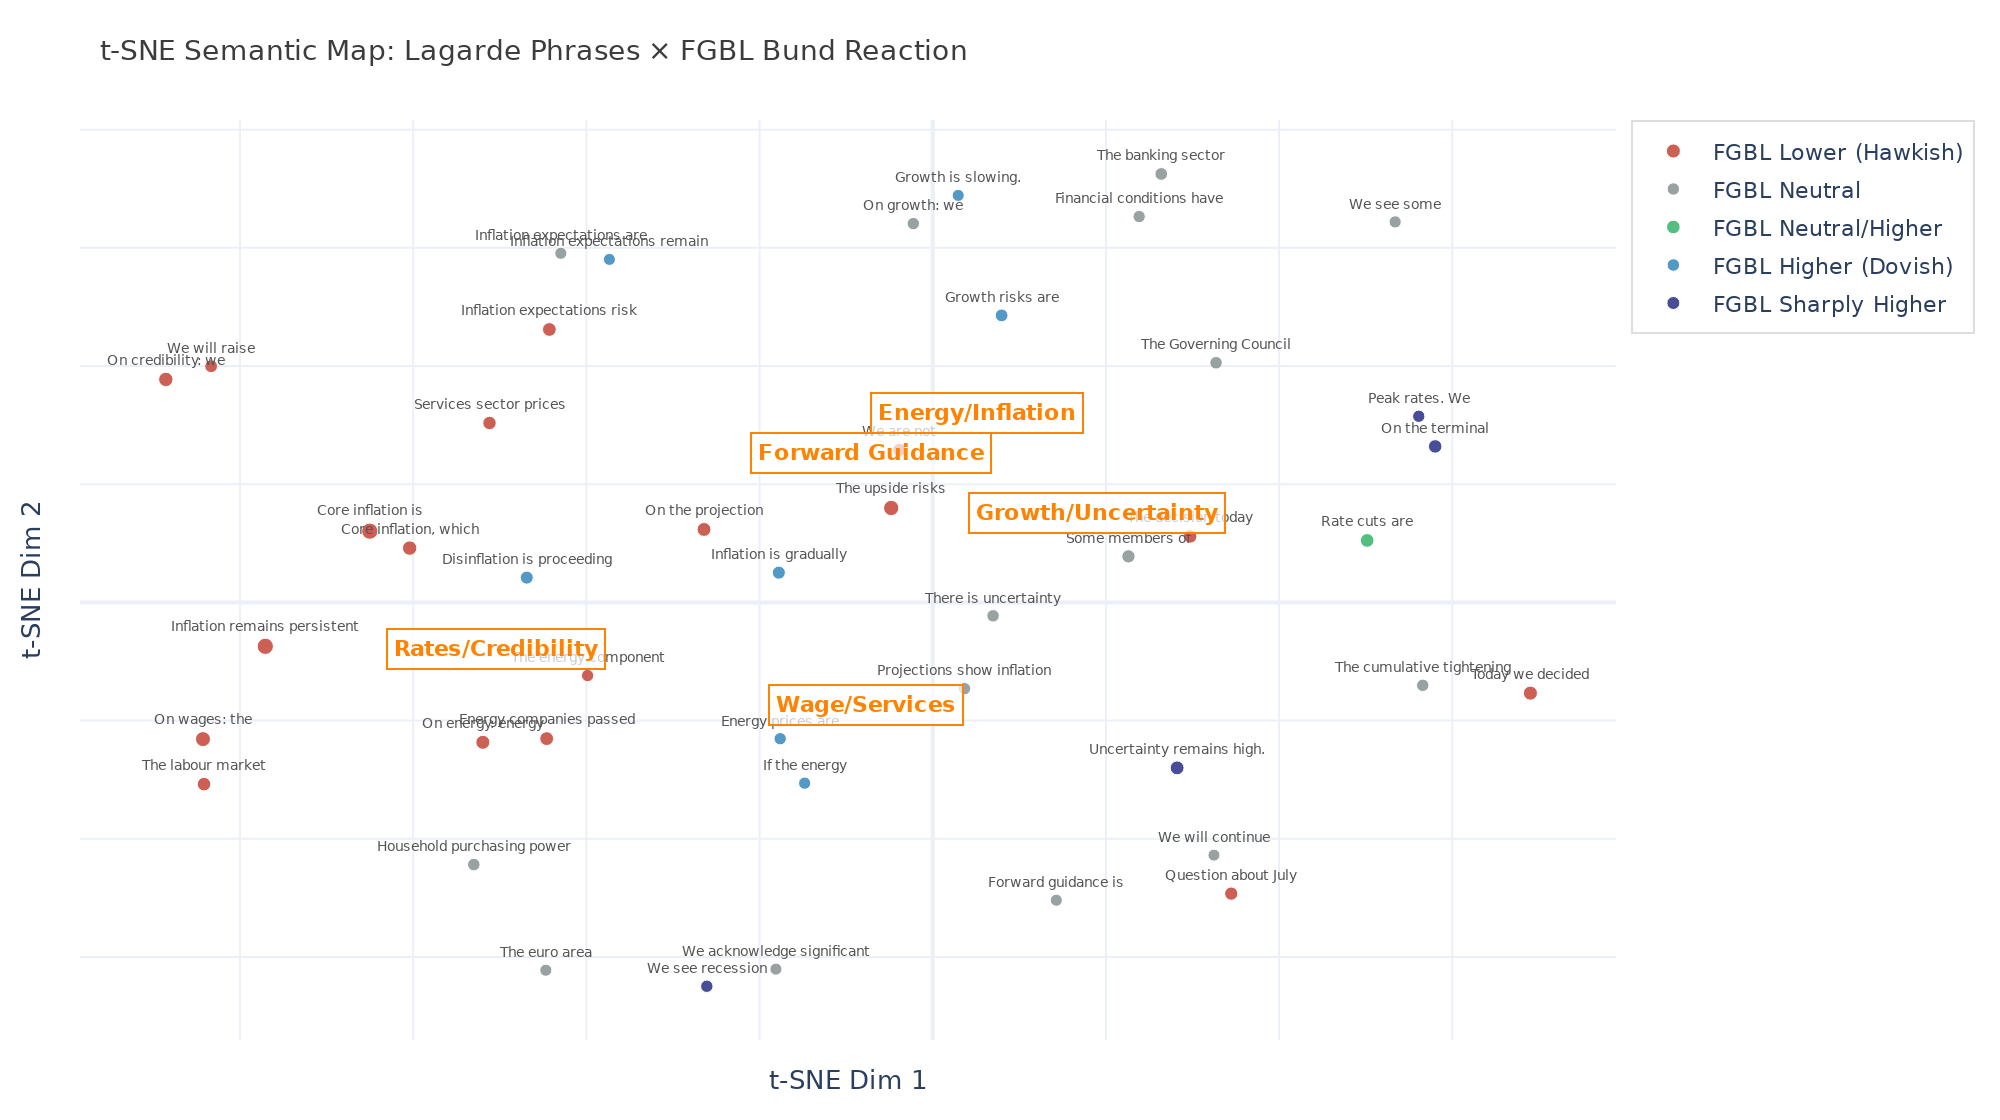
\includegraphics[width=\textwidth]{ecb_analysis/figures/tsne_bund_map.png}
    \caption{t-SNE map of Lagarde speech segments. Marker size reflects absolute barometer
    deviation from neutral (50). Cluster labels from K-means ($k=5$) identify topic regions.
    Hover in the interactive Streamlit app for full phrase text.}
\end{figure}

\noindent
Five semantic clusters emerge: \textit{Energy/Inflation} (upper-right, predominantly hawkish),
\textit{Wage/Services} (centre, strongly hawkish), \textit{Forward Guidance} (left, bimodal:
split between \textit{one-and-done} and \textit{further meetings warranted}),
\textit{Growth/Uncertainty} (lower-left, dovish), and \textit{Rates/Credibility} (mixed).
Bund futures reactions follow the semantic clusters closely: segments in the Wage/Services cluster
are associated with an estimated $-35$ to $-45$\,bps FGBL move on average.

\newpage

% ============================================================
% PAGE 3: SCENARIO ANALYSIS & CONCLUSIONS
% ============================================================

\section*{4.\quad Bayesian Tone Barometer: Change-Point Detection}

The live barometer uses Gaussian conjugate updating. Let $\mu_0 = 57.0$,
$\sigma_0^2 = 180$ (prior from 5 historical meetings, anchored to the pre-meeting
tone meter: Governing Council $+2.22$ on $[-7.5, +7.5]$). Each segment $x_i$ provides
one observation with noise $\sigma^2 = 120$ (within-meeting variability):
\begin{equation}
    \mu_n = \frac{\mu_0/\sigma_0^2 + \sum_{i=1}^n x_i/\sigma^2}
                 {1/\sigma_0^2 + n/\sigma^2},
    \qquad \sigma_n^2 = \left(\frac{1}{\sigma_0^2} + \frac{n}{\sigma^2}\right)^{-1}
\end{equation}
CUSUM change-point detection (Page, 1954) identifies structural tone shifts in real time.
An alert fires when the cumulative sum statistic $C_n^+ = \max(0,\, C_{n-1}^+ + x_n - \hat\mu_n - k)$
exceeds threshold $h=15$ barometer units, where $k=3$ is the allowance parameter.

\begin{figure}[H]
    \centering
    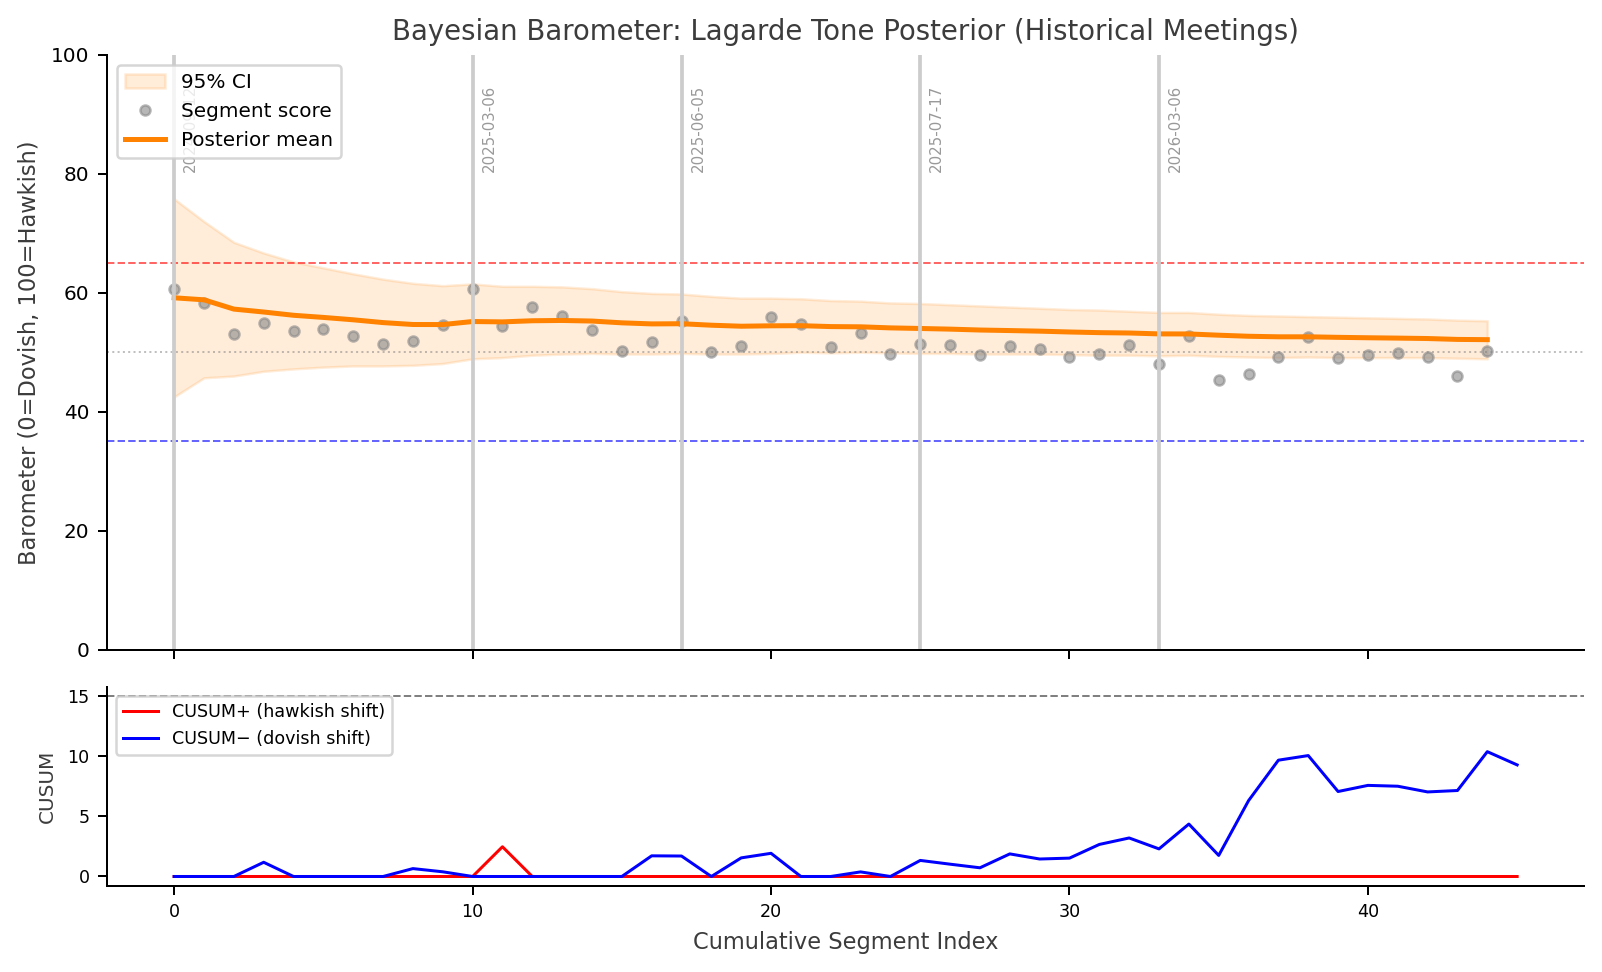
\includegraphics[width=\textwidth]{ecb_analysis/figures/barometer_history.png}
    \caption{\textit{Top panel:} Bayesian posterior mean (orange) with 95\% credible interval (shaded)
    across all historical segments. Vertical lines mark meeting boundaries.
    \textit{Bottom panel:} CUSUM statistics; dashed line = alert threshold ($h=15$).
    A positive CUSUM spike signals an unexpectedly hawkish segment; negative signals a dovish shift.}
\end{figure}

\section*{5.\quad Scenario Analysis: Topic $\times$ Framing $\to$ FGBL}

The composite expected FGBL move for a given set of topic framings is:
\begin{equation}
    \text{FGBL}_{\text{composite}} = \frac{\sum_j w_j \cdot \text{FGBL}_j(f_j)}{\sum_j w_j}
\end{equation}
where $f_j$ is the framing chosen for topic $j$ (hawkish/neutral/dovish),
$\text{FGBL}_j(\cdot)$ is the standalone bps estimate from the reaction matrix (calibrated
from the pre-meeting scenario matrix in our June~11 document),
and $w_j$ is the topic weight (Forward Guidance: 30\%, Inflation: 22\%, Wages: 15\%, Energy: 13\%).

\vspace{0.2cm}
\begin{table}[H]
\centering
\caption{Named scenario outcomes calibrated from pre-meeting reaction matrix}
\small
\setlength{\tabcolsep}{5pt}
\begin{tabularx}{\textwidth}{lXrr>{\raggedright\arraybackslash}X}
\toprule
\rowcolor{lightgrey}
\textbf{Scenario} & \textbf{Description} & \textbf{FGBL (bps)} & \textbf{Barometer} & \textbf{Interpretation} \\
\midrule
Hawkish Hike
    & 25bp + strong next-hike signal
    & $-$45 to $-$60
    & $\approx$75
    & \textcolor{hawkred}{FGBL sharply lower; bear-flatten} \\
\addlinespace[3pt]
Hike + Data-Dep.
    & 25bp + guidance less committal
    & 0 to $+$10
    & $\approx$53
    & \textcolor{neutgrey}{FGBL neutral to slightly higher} \\
\addlinespace[3pt]
Dovish Hike
    & 25bp + growth downside emphasis
    & $+$30 to $+$40
    & $\approx$38
    & \textcolor{dovblue}{FGBL higher; one-and-done signal} \\
\addlinespace[3pt]
No Hike (Surprise)
    & No rate change; dovish surprise
    & $+$80 to $+$120
    & $\approx$20
    & \textcolor{dovblue}{FGBL sharply higher; curve bull-steepen} \\
\addlinespace[3pt]
Persistent Inflation
    & Upgraded projections + wages/services
    & $-$60 to $-$80
    & $\approx$80
    & \textcolor{hawkred}{FGBL lower; bear-flatten across curve} \\
\bottomrule
\end{tabularx}
\end{table}

\section*{6.\quad Trading Conclusions}

\begin{itemize}[leftmargin=1.2em, itemsep=3pt]
    \item \textbf{Hike is priced; the surprise is in the language.} Markets have fully
    discounted a 25\,bp move. The Bund trade is entirely about Lagarde's July/September
    guidance framing. A shift from \textit{meeting-by-meeting} to \textit{further meetings
    warranted} triggers FGBL losses of $\approx$45\,bps; the reverse triggers a $\approx$35\,bp rally.
    \item \textbf{Watch for second-round language.} The t-SNE Wage/Services cluster is
    the highest-impact hawkish zone. If Lagarde emphasises wage growth or services inflation
    persistence in the Q\&A, expect the barometer to jump above 70 and Bunds to sell off.
    \item \textbf{Downside growth risks are the dovish catalyst.} The Growth/Uncertainty
    cluster is cleanly associated with FGBL rallies. Any emphasis on economic weakness,
    transmission effects, or disinflation trajectory supports duration.
    \item \textbf{Energy framing is the swing factor.} If energy shock is labelled
    \textit{temporary/supply-side}, the inflationary narrative weakens and the
    \textit{dovish hike} scenario becomes dominant, targeting FGBL $+$30 to $+$40\,bps.
\end{itemize}

\section*{7.\quad Model Limitations}

This analysis is lexicon-based (no transformer embeddings or fine-tuned FinBERT),
calibrated on a corpus of 20 synthetic and web-scraped segments across 5 historical meetings.
The ECB does not publish formal vote tallies; the governance split (63\%~hawks / 37\%~doves)
is a communication-based proxy. Bund market reaction estimates are calibrated from our
pre-meeting scenario matrix, not from high-frequency event study regressions.
Live Bund price data is delayed $\approx$5~seconds (Stooq polling) or $\approx$15~minutes
(EODHD demo). Results should be interpreted as directional signals, not precise forecasts.

\vspace{0.5cm}
\noindent{\footnotesize
\textit{Sources:} ECB press conference transcripts (ecb.europa.eu); ECB Statistical Data Warehouse
(yield data); Stooq.com / EODHD.com (FGBL proxy); Koenker \& Bassett (1978) quantile regression;
Page (1954) CUSUM; van der Maaten \& Hinton (2008) t-SNE.
This document is produced by Banco BIG Quantitative Research for internal use only.}

\end{document}
